\documentclass[a4paper,12pt]{article}

\usepackage[utf8]{inputenc}
\usepackage[T1]{fontenc}
\usepackage{graphicx}
\usepackage{geometry}
\usepackage{subcaption}
\usepackage{setspace}
\usepackage{minted}
\usepackage{authblk}
\usepackage{caption}
\usepackage{hyperref}
\usepackage{tikz}
\usetikzlibrary{trees}
\usetikzlibrary{positioning}
\usepackage{xcolor}
\usepackage{pgfkeys}
\usepackage{booktabs}
\usepackage{listings}
\usepackage[linesnumbered,ruled,vlined]{algorithm2e}
\usepackage[noend]{algpseudocode}
\usepackage{fancyhdr}
\setlength{\parindent}{0pt}
\geometry{a4paper, margin=2.5cm}

\sloppy
\begin{document}

\begin{titlepage}

    \vspace*{4cm}

    \centering
    
    
\includegraphics[width=0.6\textwidth]{Images/logo.png} \\[1.5cm]
    
    \rule{\linewidth}{1pt} \\[1cm]

    {\Huge \bfseries HAX907X Apprentissage statistique}\\[0.5cm]
    {\Huge TP : Support Vector Machines (SVM)}\\[1cm]
    
    \rule{\linewidth}{1pt} \\[2cm]

    {\Large \textbf{Marine GERMAIN}}\\
    {\Large \textbf{Coralie ROMANI DE VINCI}}\\[1cm]
    

\end{titlepage}


\renewcommand{\contentsname}{Table des matières}
\tableofcontents


\newpage

\section{Introduction}

Les \emph{Support Vector Machines} (SVM) sont une méthode de classification supervisée qui vise à séparer différentes classes en maximisant la marge entre elles. Le principe repose sur la recherche d’hyperplans séparateurs, ce qui les rend particulièrement efficaces dans des espaces de grande dimension.\\

Dans ce TP, nous mettons en pratique les SVM à l’aide du package scikit-learn. Nous appliquerons ces méthodes à la fois sur des données simulées et sur des jeux de données réels, en particulier le dataset \texttt{iris} et une base de données d'images. 
Nous analyserons également l’influence des noyaux et des hyperparamètres sur la performance des modèles, afin de mieux comprendre cette approche de classification.

\section{Base de données \texttt{iris}}

Cette section est consacrée à l'étude de la base de données \texttt{iris} sur laquelle nous ferons une étude de classification sur les classes $1$ et $2$.
Nous considérerons d'abord le noyau linéaire puis le noyau polynomial et nous les comparerons.
Le dataset est divisé en deux parties : un ensemble d'entraînement (75\% des données) et un ensemble de test (25\%). 

\subsection{Classification avec noyau linéaire}

La classification des deux premières variables avec un noyau linéaire a pour objectif de trouver un hyperplan qui sépare au mieux les deux classes en maximisant la marge entre les points des deux classes. 
Les scores obtenus pour cette méthode sont les suivants : 

\begin{figure}[H]
    \centering
    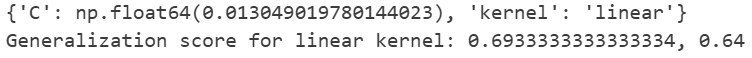
\includegraphics[width=0.8\textwidth]{Images/linear_score.png}
    \caption{Score obtenu pour le noyau linéaire}\label{fig : linear}
\end{figure}

Pour les données d'entraînement, le modèle a classifié correctement 69,3\% des données, contre 64\% pour les données de test. 


\subsection{Classification avec noyau polynomial}

L’utilisation d’un noyau polynomial sur les deux premières variables permet de trouver une frontière de décision non linéaire capable de séparer au mieux les deux classes. 
L'objectif est d'évaluer si l'emploi d'un noyau polynomial nous permet d'obtenir un meilleur classifieur que celui obtenu précédemment.\\
Les scores obtenus pour cette méthode sont les suivants :

\begin{figure}[H]
    \centering
    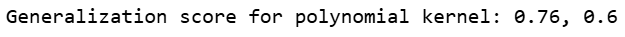
\includegraphics[width=\textwidth]{Images/poly_score.png}
    \caption{Score obtenu pour le noyau polynomial}\label{fig : poly}
\end{figure}

Pour les données d'entraînement et de test, le modèle a classifié correctement 68\% des données. \\

\textbf{Comparaison des deux méthodes  : }\\[0.5cm]
- Nous disposons d'abord des scores obtenus en figure \ref{fig : linear} et figure \ref{fig : poly}.
On remarque que le score de test obtenu pour le noyau polynomial est supérieur à celui du noyau linéaire : $0.68 \geq 0.64$.
La différence reste toutefois relativement faible, ce qui ne permet pas de conclure à une nette supériorité du modèle polynomial.\\

- Ensuite, nous avons tracé graphiquement ces résultats à l'aide des frontières : \\
\begin{figure}[H]
    \centering
    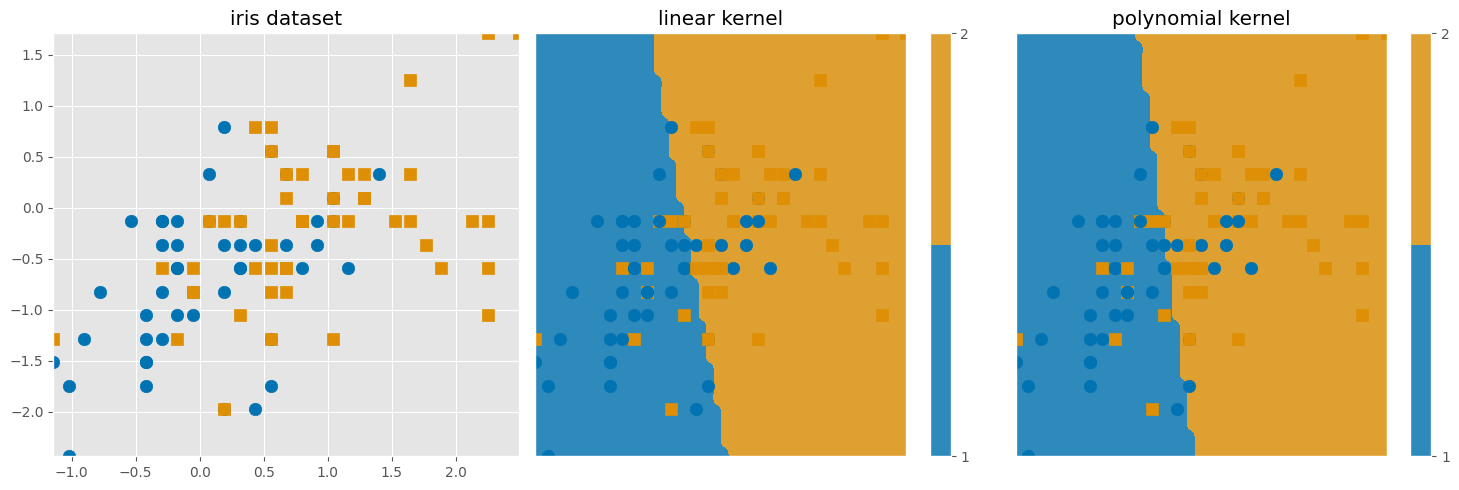
\includegraphics[width=\textwidth]{Images/linear_vs_poly.png}
    \caption{Visualisation de la frontière séparant les classes 1 (en bleu) et 2 (en orange) pour les noyaux linéaire et polynomial}\label{fig : compare}
\end{figure}

La figure \ref{fig : compare} illustre les frontières de décision obtenues par les deux classifieurs appliqués au dataset \texttt{iris}.  
On remarque que la frontière associée au noyau polynomial reste proche d’une séparation linéaire. \\
En comparant les graphiques, on constate que le classifieur linéaire commet moins d’erreurs sur les données de la classe 1, tandis que le classifieur polynomial en commet moins sur les données de la classe 2.  \\
À ce stade, les performances des deux modèles semblent similaires, sans qu’un noyau ne se démarque nettement de l’autre.

\newpage

\section{SVM GUI}

Nous utilisons dans cette section le script \texttt{svm\_gui.py}  permettant de lancer une application qui évalue en temps réel l’impact du choix du noyau et du paramètre de régularisation C.
Nous avons généré manuellement deux jeux de données très déséquilibrée, un de 90 données et l'autre de 10 données. 
À l'aide d'un noyau linéaire et en faisant évoluer la valeur de C, nous obtenons la figure \ref{fig : carre}.


\begin{figure}[H]
    \centering
    \begin{subfigure}[b]{0.45\textwidth}
        \centering
        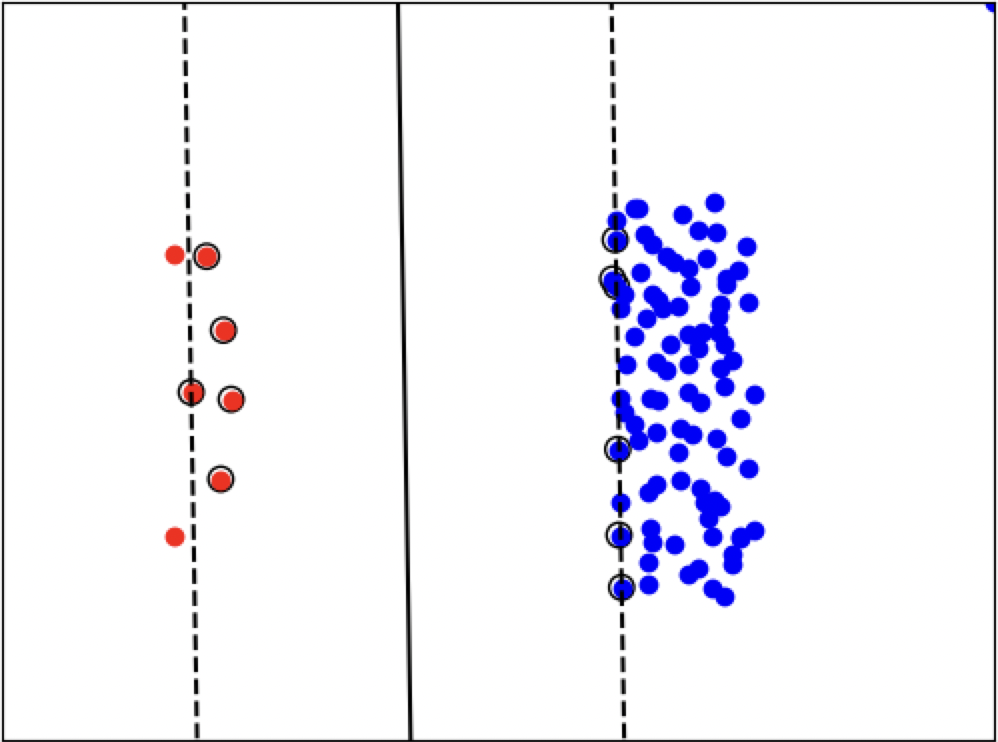
\includegraphics[width=\textwidth]{Images/C=1.png}
        \caption{C = 1 (pour 90 données)}
    \end{subfigure}
    \hfill
    \begin{subfigure}[b]{0.45\textwidth}
        \centering
        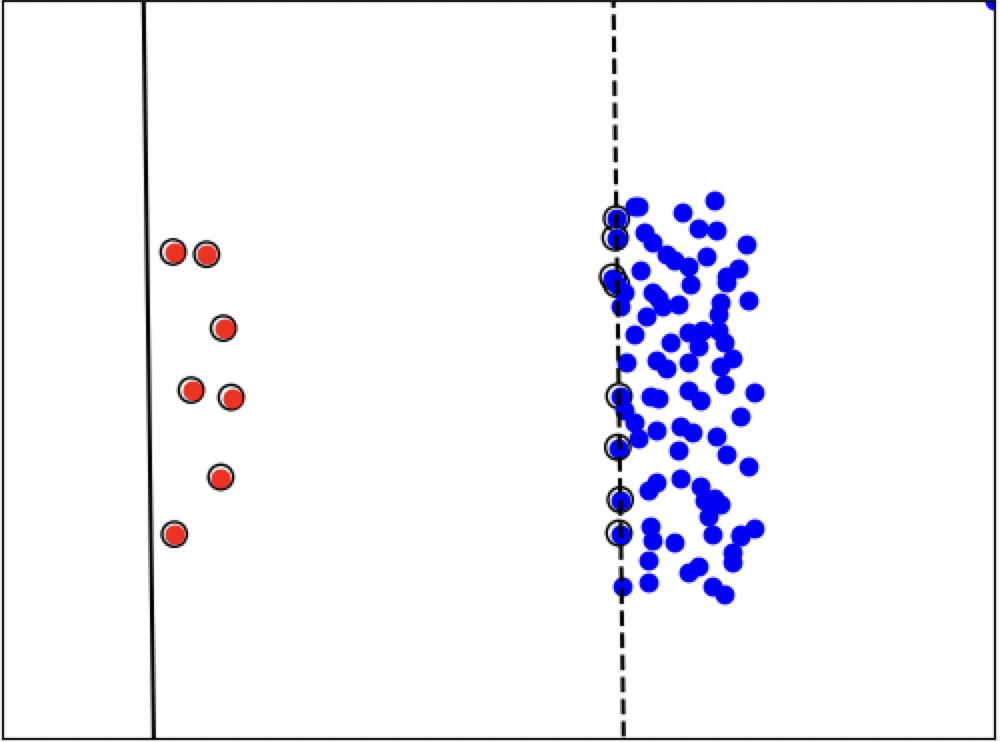
\includegraphics[width=\textwidth]{Images/C=0.3.png}
        \caption{C = 0.3 (pour 90 données)}
    \end{subfigure}

    \begin{subfigure}[b]{0.45\textwidth}
        \centering
        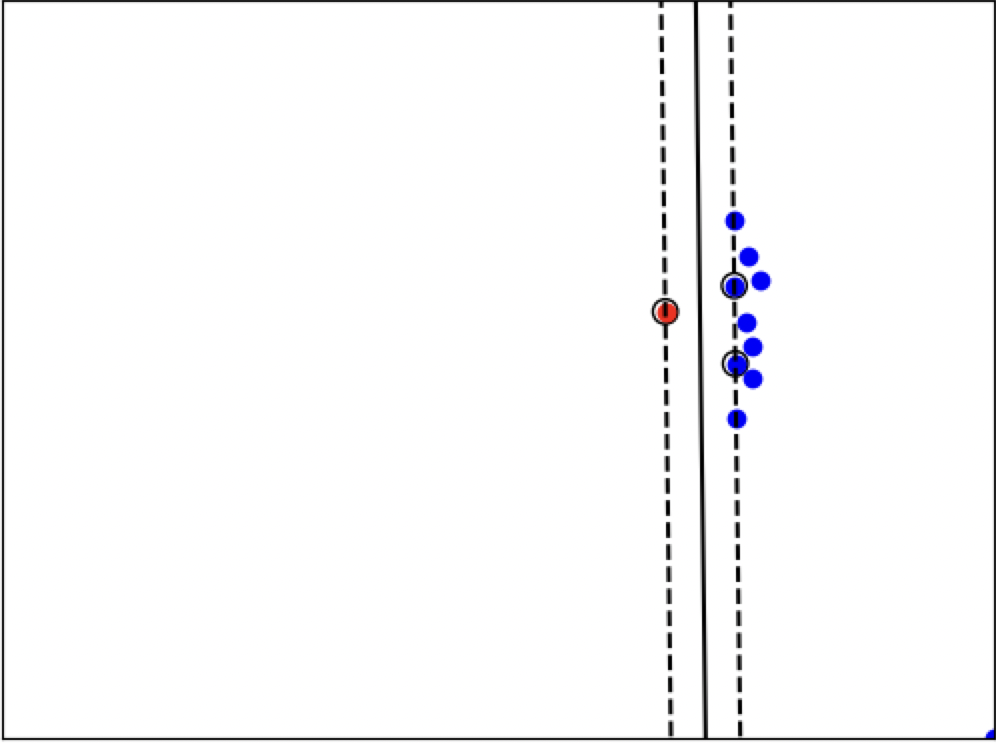
\includegraphics[width=\textwidth]{Images/C=10.png}
        \caption{C = 10 (pour 10 données)}
    \end{subfigure}
    \hfill
    \begin{subfigure}[b]{0.45\textwidth}
        \centering
        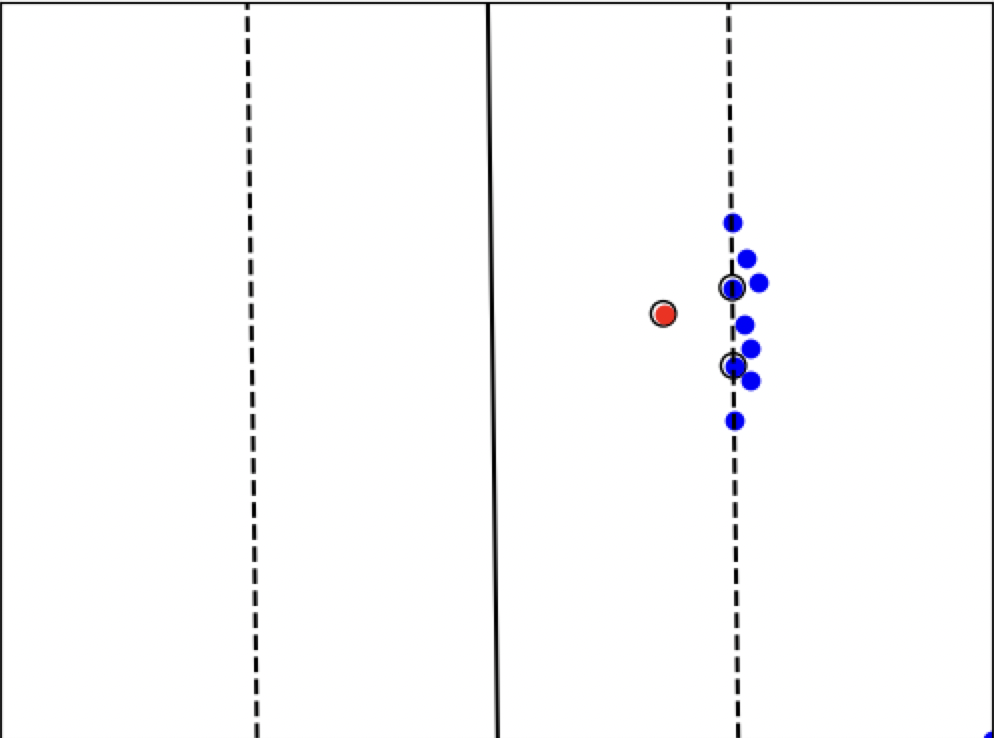
\includegraphics[width=\textwidth]{Images/C=1_bis.png}
        \caption{C = 1 (pour 10 données)}
    \end{subfigure}

    \caption{Visualisation de la région de décision selon différents paramètres de régularisation C}\label{fig : carre}
\end{figure}

L'influence du paramètre de régularisation est similaire pour les deux jeux de données, mais pas aux mêmes ordres de grandeur.

\begin{itemize}
    \item Pour un grand jeu de données (voir figure (a) et (b)) : L'influence de C est visible à une échelle de $10^{-1}$.
    \item Pour un petit jeu de données (voir figure (c) et (d)) : L'influence de C est visible à une échelle de $1$ (à noter que pour $C \leq 1$, il n'y a pas de changement visible).
\end{itemize}

Dans les deux cas, on remarque que lorsque C diminue, la frontière de décision et les marges évoluent en fonction de la classe majoritaire.
En effet, plus C diminue plus les marges sont imprécises en s'élargissant jusqu'à ce que toutes les observations soient classées du même côté.
\newpage

\section{Classification des visages}

Dans cette section, nous exploitons une base d'images extraites de « Labeled Faces in the Wild ».
L'objectif est de classifier, à l'aide d'un SVM à noyau linéaire, deux types d'images : des portraits de Tony Blair (figure \ref{fig : visages}) et de Colin Powell. 


\begin{figure}[H]
    \centering
    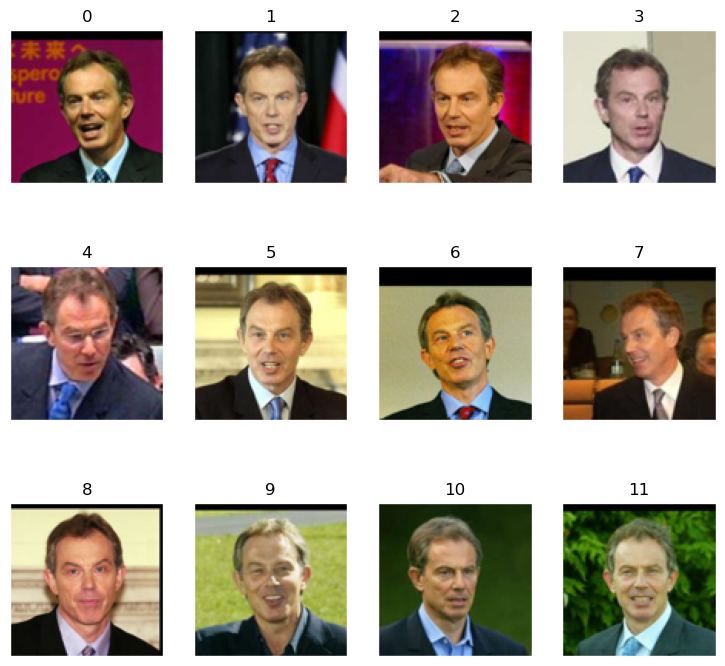
\includegraphics[width=0.6\textwidth]{Images/visages.png}
    \caption{Base de données de 12 portraits de Tony Blair}\label{fig : visages}
\end{figure}

\subsection{Influence du paramètre de régularisation}

Nous souhaitons observer l'influence du paramètre de régularisation $C$ sur la qualité du classifieur. 
Pour cela, nous estimons le score d'apprentissage en fonction de ce paramètre à la figure \ref{fig : C}.

\begin{figure}[H]
    \centering
    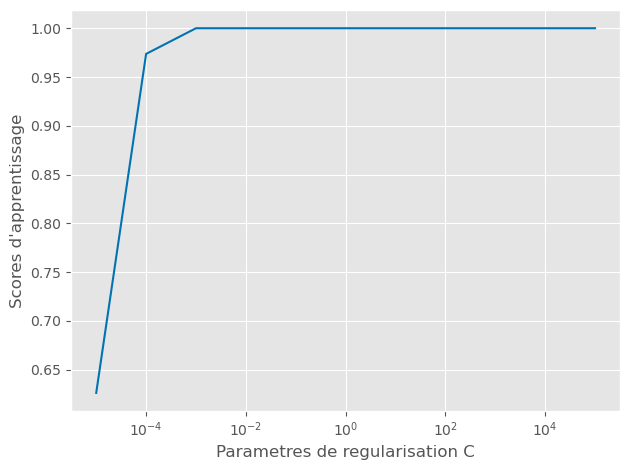
\includegraphics[width=0.6\textwidth]{Images/erreur_prediction.png}
    \caption{Score d'apprentissage en fonction du paramètre de régularisation C pour des classifieurs SVM à noyau linéaire}\label{fig : C}
\end{figure}

En faisant varier les valeurs de C entre $10^{-5}$ et $10^{5}$, on remarque qu'on atteint un score d'apprentissage maximal d'environ $0.725$ lorsque $C=10^{-1}$.
Au delà de cette valeur de C, le score reste maximal de façon constante.\\
Ce résultat est cohérent, car il est attendu qu’un SVM atteigne un score maximal pour une valeur intermédiaire de 
C. En effet, si C est trop petit il y a un risque un sous-apprentissage et s'il est trop grand, il y a un risque de sur-apprentissage.\\
Ainsi, le paramètre de régularisation optimal est $C=0.1$.\\[0.5cm]


\begin{figure}[H]    
    \centering    
    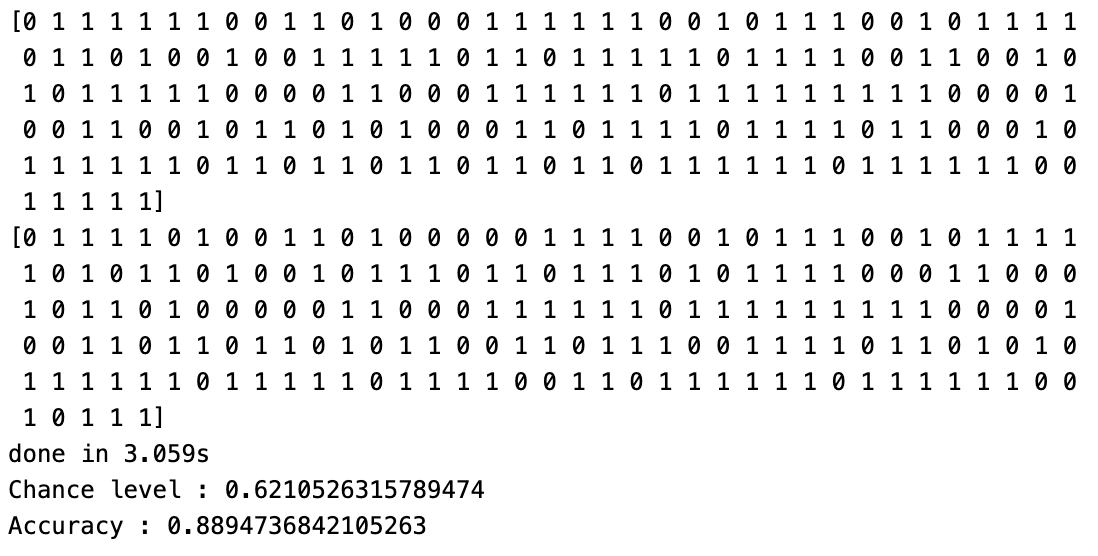
\includegraphics[width=0.8\textwidth]{Images/label_prediction.png}
    \caption{Visualisation de la prédiction du test et de sa précision}\label{fig : precision}
\end{figure}

La figure \ref{fig : precision} illustre les résultats obtenus avec le classifieur SVM linéaire optimal : 
\begin{itemize}
    \item Prédiction : matrice binaire des valeurs prédites pour les images par le classifieur entraîné.
    \item Test : matrice binaire des valeurs réelles correspondant aux images.
\end{itemize}

Ainsi, le classifieur linéaire atteint une précision nettement supérieure au niveau de chance, démontrant sa capacité à distinguer correctement les classes sur ce jeu de test.

\begin{figure}[H]
    \centering
    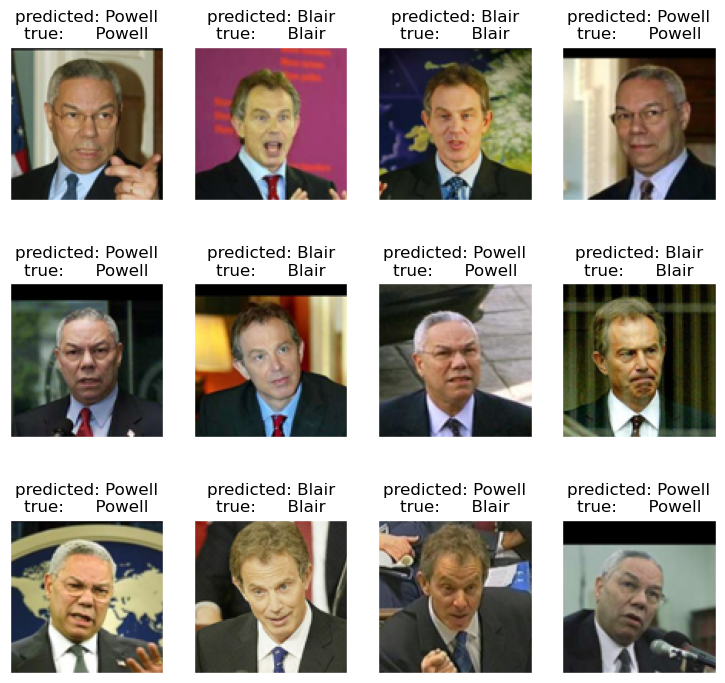
\includegraphics[width=0.6\textwidth]{Images/prediction_visage.png}
    \caption{Prédictions faites à partir du classifieur optimal sur un échantillon d'images}\label{fig:predict}
\end{figure}

La figure \ref{fig:predict} montre un échantillon des résultats obtenues : sur 12 images, 11 ont été correctement prédites, ce qui correspond environ à 91\% de bonnes réponses.

\begin{figure}[H]
    \centering
    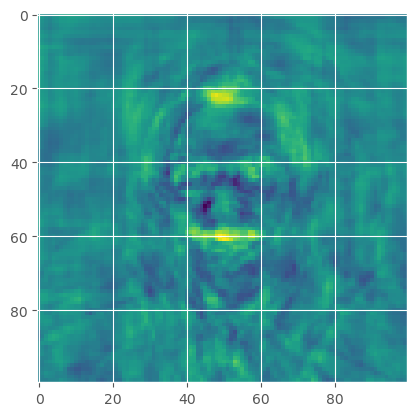
\includegraphics[width=0.5\textwidth]{Images/coeff_visage.png}
    \caption{Visualisation des coefficients du SVM}\label{fig : ?}
\end{figure}

La figure \ref{fig : ?} permet de visualiser les coefficients du SVM sous la forme d'une image.
Cela colore différemment les zones influençant le SVM vers chaque classe. 
En effet, les zones très claires (jaune) pousseront vers une classe, tandis que que les zones très foncées (violet) pousseront vers l'autre classe.
Les zones vertes n'influenceront pas ou très peu la décision du SVM.

\subsection{Variable de nuisances}

Nous voulons maintenant, montrer que le score de prédiction est sensible au bruit. Pour cela, nous ajoutons des variables de bruit et
recommençons la prédiction. Le bruitage consiste à ajouter des variables de bruit (ici 300), et à les mélanger aux autres. 

Nous obtenons alors les valeurs suivantes avec et sans nuisances :

\begin{figure}[H]
    \centering
    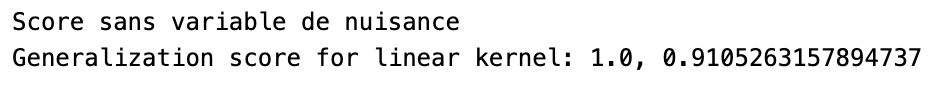
\includegraphics[width=0.8\textwidth]{Images/sans_variable.png}
    \caption{Score sans variable de nuisance}\label{fig: sans}
\end{figure}

\begin{figure}[H]
    \centering
    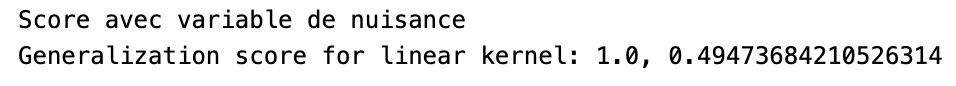
\includegraphics[width=0.8\textwidth]{Images/avec_variable.png}
    \caption{Score avec variable de nuisance}\label{fig: avec}
\end{figure}

Nous constatons que le bruit endommage fortement le classifieur qui voit son score presque réduit de moitié.

\subsection{Réduction de dimensions}

À présent, nous voulons améliorer la prédiction obtenue dans la question précédente (figure \ref{fig: avec}) à l'aide d'une ACP.

\begin{figure}[H]
    \centering
    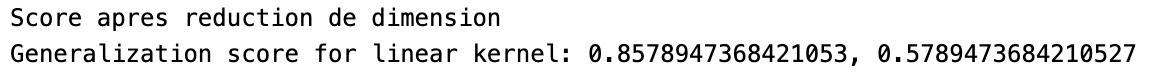
\includegraphics[width=0.8\textwidth]{Images/apres_reduction.png}
    \caption{Scores obtenus pour n=90}\label{fig : dim}
\end{figure}

\begin{figure}[H]
    \centering
    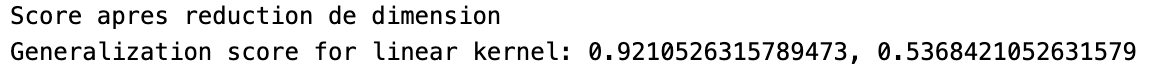
\includegraphics[width=0.8\textwidth]{Images/n=200.png}
    \caption{Scores obtenus pour n=200}\label{fig : dim2}
\end{figure}

Pour commencer, on doit choisir le nombre de composantes $n$ optimales qui équilibre le mieux l'information reçue et le bruit conservé.
Dans notre cas, on s'est rendu compte que lorsque $n$ est trop petit (à partir de $n = 70$), l'algorithme tourne à l'infini. On suppose qu'un  nombre de dimension trop faible empêche la convergence du SVM.\\
On a ensuite, testé pour $n = 90$ et pour $n = 200$. On remarque que les scores de test sont très proches néanmoins, lorsque $n$ est trop grand (figure \ref{fig : dim2}) le score n'est pas fiable en raison du grand nombre de bruits conservés.\\
\\
Finalement, il existe une solution pour améliorer le score d'un jeu de données bruité : la réduction de dimension. Dans notre cas, le choix de $n = 90$ nous semble intéressant car on passe d'un score de 0.49 à 0.54.
Ce changement n'est pas significatif (seulement +5\%) car à 90 composantes il reste toujours du bruit.

\subsection{Biais dans le prétraitement des données}

Malgré les résultats obtenus précédemment, il existe un biais dans notre prétraitement. 
En effet, les données ont été standardisées avant leur séparation en ensembles d'entraînement et de test.
Cela signifie que les statistiques utilisées pour normaliser l'ensemble d'entraînement ont été calculées en incluant l'ensemble de test. 
Le modèle possède alors indirectement des informations provenant des données de test, ce qui surestime ses performances réelles.
\\
AJOUTER LES LIGNES DE CODE CORRESPONDANTES
PARLER DE FUITE DE DONNÉES OU DE DATA LEAKAGE
\end{document}
